\documentclass{beamer}
\usepackage{tfrupee} % Include tfrupee package
\usepackage{amsmath,amssymb,amsfonts,amsthm}
\usepackage{graphicx}
\usepackage{enumitem}
\usepackage{mathtools}
\usepackage{gensymb}
\usepackage{minted}
\title{Construction of triangle}
\author{AI24BTECH11006 - Bugada Roopansha}
\institute{IIT Hyderabad}
\date{November 6, 2024}

\begin{document}

\begin{frame}
    \titlepage
\end{frame}

\begin{frame}{Question}
    \textbf{Construct a right triangle when one side is 3.5 cm, and the sum of the other side and the hypotenuse is 5.5 cm.}
    
\end{frame}

\begin{frame}{Solution: Parameters}
    \begin{table}[h!]
        \centering
        \begin{tabular}{|c|c|c|}
            \hline
            \textbf{Segment} & \textbf{Norm} & \textbf{Angles} \\ \hline
            \( ||AB|| \) & 3.5 & $\angle{C}$ \\ \hline
            \( ||BC|| \) & Distance between B and C & $\angle{A}=90\degree$ \\ \hline
            \( ||AC||\) & Distance between C and A & $\angle{B} $ \\ \hline
        \end{tabular}
        \caption{Input parameters}
    \end{table}
\end{frame}

\begin{frame}{Solution:}
    Given:
    \[
    c = 3.5 \, \text{cm}, \quad a + b = 5.5 \, \text{cm},\quad \angle{A}=90\degree
    \]
    Using the cosine formula in $\triangle ABC$
    
    \[
    a^2 = b^2+c^2-2bc \cos A
    \]
    
    \[
    \implies (5.5 - b)^2 = b^2+c^2 -2bc \cos A
    \]
\end{frame}

\begin{frame}{Solution: Further Calculations}
    Expanding and solving the equation :
    \[
    \implies b \approx 2.5cm
    \]
    
    The coordinates of $\triangle ABC$ can then be expressed as:
    \[
    C=b \begin{bmatrix} \sin A \\ \cos A \end{bmatrix}, \quad
    A=0 \quad
    B=  \begin{bmatrix} 0 \\ c \end{bmatrix}
    \]
\end{frame}


\begin{frame}[fragile]
\frametitle{C-Code}
\begin{minted}[bgcolor=bg, linenos, fontsize=\small, breaklines]{c}
  #include <stdio.h>
#include <math.h>

int main() {
    // Given values
    double a = 3.5;        // One side of the triangle
    double sum_bc = 5.5;   // Sum of the other side and the hypotenuse

    // Variables to hold the lengths of the other side and the hypotenuse
    double b, c;

    // Calculate the other side (b) and the hypotenuse (c)
    b = (pow(sum_bc, 2) - pow(a, 2)) / (2 * sum_bc);
    c = sum_bc - b;

   

\end{minted}
\end{frame}
\begin{frame}[fragile]
\frametitle{C-Code}
\begin{minted}[bgcolor=bg, linenos, fontsize=\small, breaklines]{c}
  // Calculate the endpoints
    double Ax = 0.0, Ay = 0.0;         // Vertex A
    double Bx = 0.0, By = a;            // Vertex B
    double Cx = b, Cy = 0.0;            // Vertex C

    // Open a file for writing
    FILE *file = fopen("data.txt", "w");
    if (file == NULL) {
        printf("Error opening file!\n");
        return 1;
    }

    // Write the endpoints to the file
    fprintf(file, "Endpoints of the triangle:\n");
    fprintf(file, "A (0.00, 0.00)\n");
    fprintf(file, "B (0.00, %.2f)\n", By);
    fprintf(file, "C (%.3f, 0.00)\n", Cx);

   
\end{minted}
\end{frame}

\begin{frame}[fragile]
\frametitle{C-Code}
\begin{minted}[bgcolor=bg, linenos, fontsize=\small, breaklines]{c}
  // Close the file
    fclose(file);

    // Output to console (optional)
    printf("Endpoints saved to data.txt\n");
    printf("A (%.2f, %.2f)\n", Ax, Ay);
    printf("B (%.2f, %.2f)\n", Bx, By);
    printf("C (%.3f, %.2f)\n", Cx, Cy);

    return 0;
}
\end{minted}
\end{frame}
\begin{frame}[fragile]
\frametitle{Python Code}
\begin{minted}[bgcolor=bg, linenos, fontsize=\small, breaklines]{c}
  import numpy as np
import matplotlib.pyplot as plt

# Function to read coordinates from 'data.txt'
def read_coordinates(filename='data.txt'):
    coordinates = {}
    with open(filename, 'r') as file:
        for line in file:
            line = line.strip()  # Remove any leading/trailing whitespace
            if line:  # Skip empty lines
                try:
                    point, coords = line.split(' ', 1)  # Split into point and coordinates
                    coords = coords.strip('()')  # Remove parentheses
                    x, y = map(float, coords.split(','))  # Split by ',' and convert to floats
                     
\end{minted}
\end{frame}
\begin{frame}[fragile]
\frametitle{Python Code}
\begin{minted}[bgcolor=bg, linenos, fontsize=\small, breaklines]{c}
                    
                    coordinates[point] = np.array([x, y]).reshape(-1, 1)
                except ValueError as e:
                    print(f"Error processing line: {line}. Error: {e}")
    return coordinates

# Read triangle vertices from 'data.txt'
vertices = read_coordinates()

# Check if vertices were read correctly
if not vertices:
    print("No vertices found. Exiting.")
    exit()

# Extract points A, B, and C from the vertices
A = vertices['A']
B = vertices['B']
\end{minted}
\end{frame}
\begin{frame}[fragile]
\frametitle{Python Code}
\begin{minted}[bgcolor=bg, linenos, fontsize=\small, breaklines]{c}

C = vertices['C']

# Function to generate the line between two points
def line_gen(P, Q):
    return np.hstack((P, Q))

# Generate lines for the triangle sides
x_AB = line_gen(A, B)
x_BC = line_gen(B, C)
x_CA = line_gen(C, A)

# Plotting the triangle sides
plt.plot(x_AB[0, :], x_AB[1, :], label='AB')
plt.plot(x_BC[0, :], x_BC[1, :], label='BC')
plt.plot(x_CA[0, :], x_CA[1, :], label='CA')

\end{minted}
\end{frame}
\begin{frame}[fragile]
\frametitle{Python Code}
\begin{minted}[bgcolor=bg, linenos, fontsize=\small, breaklines]{c}
# Scatter plot of the vertices
plt.scatter(A[0], A[1], color='red', zorder=5)
plt.scatter(B[0], B[1], color='red', zorder=5)
plt.scatter(C[0], C[1], color='red', zorder=5)
# Label the vertices with coordinates
plt.text(A[0] + 0.1, A[1], f'A {A.flatten()}', fontsize=12, ha='center')
plt.text(B[0] + 0.1, B[1], f'B {B.flatten()}', fontsize=12, ha='center')
plt.text(C[0] + 0.1, C[1], f'C {C.flatten()}', fontsize=12, ha='center')
# Set equal scaling and labels
plt.axis('equal')
plt.xlabel('x')
plt.ylabel('y')
plt.grid(True)
plt.legend()
plt.title('Triangle ABC with Coordinates')
# Show the plot
plt.show()

\end{minted}
\end{frame}
\begin{frame}{Diagram}
    \begin{figure}[h!]
        \centering
        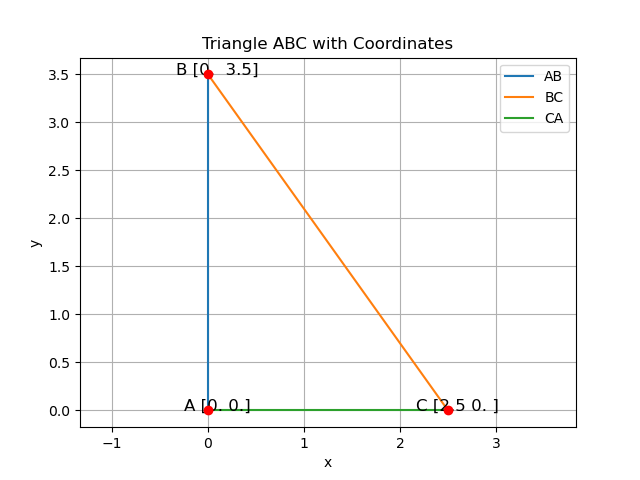
\includegraphics[width=0.9\textwidth]{fig.png} % Replace with your triangle diagram
        \caption{Right triangle with  c= 3.5 cm , a+b= 5.5 cm and $\angle{A}=90\degree$.}
    \end{figure}
\end{frame}

\end{document}


